\documentclass[a4paper,polish,12pt]{article}
    \usepackage[utf8]{inputenc}
    \usepackage[T1]{fontenc}
    \usepackage{lmodern}
	\usepackage{amsmath}
	\usepackage{xcolor}
    \usepackage{babel}
    \usepackage{csquotes}
    \DeclareQuoteAlias{croatian}{polish}
   \usepackage{hyperref}
 
\usepackage{graphicx}
\title{Dokumentacja}
\author{Mateusz Banaszek \and Szymon Kozakiewicz \and Joanna Świętosławska}
\begin{document}
\maketitle
\section{Zespól i jego zadania}
Zespół projektowy składał się z 3 osób.  Podział obowiązków był następujący:\\
Mateusz Banaszek - nadzorowanie postepów projektu, testy, dokumentacja,\\
Szymon Kozakiewicz - programowanie I,\\
Jaonna świetosławka - programowanie II.


\begin{figure}


\label{zdj:2}
\centering
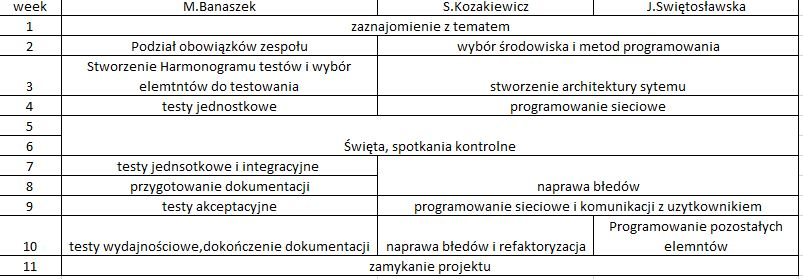
\includegraphics[width=\textwidth]{1.jpg}
\caption{Wykres Gantta.}
\end{figure}

Przegląd posępu prac prezentuje diagram Gantta( patrz rys. \ref{zdj:2}). 

\section{Opis programu}
Program ma za zadanie udostępniać interfejs do komunikacji z full nodem sieci bitcoin. Pozawala na nawiązanie z nim połączenie oraz podstawową wymianę danych. Można więc uzyskać informacje o adresach innych węzłów czy otrzymać informacje o blokach i ich zawartości. Udostępnia też wysyłanie wiadomości czysto serwisowych takich jak ping, version czy verack. Możliwe są też różne sposoby na nawiązanie połączenia czyli UDP i TCP. 

\subsection{Realizowane funkcjonalności}

\begin{itemize}


\item Ustanowienie połączenia
\begin{itemize}
\item TCP
\item UDP
\end{itemize}

\item Komunikacja z użytkownikiem za pomocą konsoli
\item Znajdywanie adresów ip węzłów za pomocą DNS seed
\item Wysyłanie wiadomości:
\begin{itemize}
\item getaddr
\item addr
\item version
\item verack
\item ping
\item inv
\item getdata
\item getblocks
\end{itemize} 
\item Odbiór wiadomości
\begin{itemize}
\item addr
\item version
\item verack
\item ping
\item inv
\item tx

\end{itemize}
\end{itemize}
\subsection{Uruchomienie programu}
\label{chap:1}
By uruchomić program należy wywołać polecenie $$python3 Console.py$$
Aplikacja była testowana dla pythona w wersji 3.6 na innych wersjach może on nie działać poprawnie.
\subsection{Opis działania}

Po uruchomieniu programu do konsoli można wpisać następujące polecenia:
\begin{itemize}
\item \textit{ping}:* wysyła wiadomość ping do wybranego hosta.
\item \textit{polacz}:* ustanawia połączenie z wybranym węzłem. Jeśli wcześniej żaden adres ip nie był ustawiony użytkownik zostanie poproszony o jego podanie. Wykonanie polecenia skutkuje wysłaniem do docelowego węzła wiadomości version. Następnie odebrana zostaje zwrotna wiadomość version od węzła. Na koniec następuje wymiana wiadomościami verack. Jeżeli nie uda się nawiązać połączenia TCP w przeciągu 5 sekund to próba połączenia kończy się niepowodzeniem.
\item \textit{help}:* Wyświetla możliwe do wpisania polecenia
\item \textit{ustaw adres}:* ustawia adres docelowego węzła
\item \textit{dns}:* wyszukiwanie adresów węzłów za pomocą dns. Wyszukane węzły zostają wypisane.
\item \textit{getaddr}: uzyskanie adresów innych węzłów z wybranego węzła
\item \textit{addr}: wysyła wiadomość addr do wybranego węzła
\item \textit{getblocks}: wyświetla bloki wybranego węzła(i hashe)
\item \textit{getdata}:  wyświetla dane z wybranego bloku. Użytkownik musi wcześniej podać hash identyfikujący wybrany blok.
\item \textit{inv}: Wysyła wiadomość inv
\end{itemize}

Uwaga! Tylko polecenia oznaczone gwiazdką da się wykonać bez wcześniejszego nawiązania połączenia z węzłem(za pomocą polecenia \textit{polacz})

\section{Implementacja}
Aplikacja została stworzona przy użyciu języka \textit{python} w wersji 3.6. Nie były używane żadne zewnętrzne biblioteki.
\subsection{Opis konstrukcji poszczególnych wiadomości}

\subsubsection{Nagłówek wiadomości}
Każda wiadomość protokołu bitcoin musi rozpoczynać się od nagłówka. Składa się on z pól przedstawionych w tabeli \ref{tab:naglowek}
\subsubsection{Adres}
w wielu wiadomościach trzeba wysłać adres ip. Zawartość części wiadomości z adresem zaprezentowano w tabeli \ref{tab:addrInet}.
\begin{table}[]
\centering
\begin{tabular}{|l|c|c|}
\hline
\multicolumn{1}{|c|}{\textbf{nazwa pola}} & \textbf{liczba bajtów} & \textbf{komentarz}                                                                                                                                                                            \\ \hline
time                                      & 4                      & \begin{tabular}[c]{@{}c@{}}Czas. Pole nie jest obecne gdy \\ adres jest częścią wiadomości\\ version\end{tabular}                                                                             \\ \hline
services                                  & 8                      & -                                                                                                                                                                                             \\ \hline
ipv6/4                                    & 16                     & \multicolumn{1}{l|}{\begin{tabular}[c]{@{}l@{}}Pierwsze 12 bajtów przechowuje adres ipv6\\ pozostałe 4 bajty trzymają ipv4. W naszej\\ implementacji wykorzystujemy tylko ipv4.\end{tabular}} \\ \hline
port                                      & \multicolumn{1}{l|}{2} & \multicolumn{1}{l|}{Numer portu}                                                                                                                                                              \\ \hline
\end{tabular}
\caption{Zawartość adresu internetowego}
\label{tab:addrInet}
\end{table}

\subsubsection{Version}
Wiadomość version składa się z pól przedstawionych w tabeli \ref{tab:version}. Wiadomość wysyłana jest w celu ustalenia zasad komunikacji.

\begin{table}[]
\centering
\begin{tabular}{|l|c|l|}
\hline
\textbf{nazwa pola} & \textbf{liczba bajtów} & \textbf{Opis}                                                                                                                              \\ \hline
magic letters       & 4                      & \begin{tabular}[c]{@{}l@{}}Każda wiadomość rozpoczyna się od tzw \\ liczb magicznych.Zwykle mają \\ one postać f9beb4d9 (hex)\end{tabular} \\ \hline
command             & 12                     & Zawiera nazwę wiadomości                                                                                                                   \\ \hline
length              & 4                      & \begin{tabular}[c]{@{}l@{}}Długość wiadomości w \\ bajtach z pominięciem nagłówka\end{tabular}                                             \\ \hline
checksum            & 4                      & Suma kontrolna(przez nas nie odczytywana)                                                                                                  \\ \hline
\end{tabular}
\caption{Zawartość nagłówka wiadomości}
\label{tab:naglowek}
\end{table}


\begin{table}[]
\centering
\begin{tabular}{|l|c|c|}
\hline
\multicolumn{1}{|c|}{\textbf{nazwa pola}} & \textbf{liczba bajtów} & \textbf{Opis}                                                                                                                \\ \hline
version                                   & 4                      & \begin{tabular}[c]{@{}c@{}}Wskazuje wersje protokołu używaną\\ przez wysyłającego. W naszym wypadku \\ było to 60002\end{tabular} \\ \hline
services                                  & 8                      & -                                                                                                                                 \\ \hline
timestamp                                 & 8                      & czas wysłania wiadomości                                                                                                          \\ \hline
addr\_recv                                & 26                     & Adres adresata wiadomości                                                                                                         \\ \hline
addr\_from                                & 26                     & Adres wysyłającego                                                                                                                \\ \hline
nonce                                     & 8                      & -                                                                                                                                 \\ \hline
user\_agent                               & ?                      & -                                                                                                                                 \\ \hline
start\_height                             & 4                      & -                                                                                                                                 \\ \hline
relay                                     & 1                      & -                                                                                                                                 \\ \hline
\end{tabular}
\caption{Zawartość wiadomości version}
\label{tab:version}
\end{table}
\subsubsection{Verack}
Wiadomość składa się z samego nagłówka. Wysyłana jest w celu potwierdzenia nawiązania komunikacji.
\subsubsection{Getaddr}
Wiadomość składa się z samego nagłówka. Wysyłana jest w celu uzyskania nowych adresów ip węzłów.
\subsubsection{Addr}
Zawartość wiadomości addr została przedstwaiona w tabeli \ref{tab:addr}
\begin{table}[]
\centering
\begin{tabular}{|l|c|c|}
\hline
\multicolumn{1}{|c|}{\textbf{nazwa pola}} & \textbf{liczba bajtów} & \textbf{komentarz}                                                                                                                                                                                         \\ \hline
count                                     & 1+                     & \begin{tabular}[c]{@{}c@{}}Określa liczbę adresów wysłanych\\ wraz z wiadomością. Wykorzystywany jest tu \\ typ danych zwany varint dlatego nie można\\ jednoznacznie określić wielkości pola\end{tabular} \\ \hline
addr\_list                                & ?                      & \begin{tabular}[c]{@{}c@{}}Lista adresów wysyłanych w \\ wiadomości\end{tabular}                                                                                                                           \\ \hline
\end{tabular}
\caption{Zawartość wiadomości addr}
\label{tab:addr}
\end{table}
\subsubsection{Getblocks}
Wiadomość getblocks składa się z pól przedstawionych w tabeli \ref{tab:getblocks}. Wysłanie tej wiadomości jest równoznaczne z~zarządaniem odpowiedzi w~postaci wiadomości inv.

\begin{table}[]
\centering
\begin{tabular}{|l|c|c|}
\hline
\multicolumn{1}{|c|}{\textbf{nazwa pola}} & \textbf{liczba bajtów} & \textbf{Opis}                                                                                                                \\ \hline
version                                   & 4                      & \begin{tabular}[c]{@{}c@{}}Wskazuje wersje protokołu używaną\\ przez wysyłającego. W naszym wypadku \\ było to 60002\end{tabular} \\ \hline
liczba hashy                               & 1+                     & -                                                                                                                                 \\ \hline
hashe nagłówków bloków                                & 32*liczba hashy                      &                                                                                               \\ \hline
hash stopu                               & 32                    & Hash składający się z~samych zer                                                                                                       \\ \hline
\end{tabular}
\caption{Zawartość wiadomości getblocks}
\label{tab:getblocks}
\end{table}

\subsubsection{Getdata}
Wiadomość getblocks składa się z pól przedstawionych w tabeli \ref{tab:getdata}. Wysłanie tej wiadomości jest równoznaczne z~zarządaniem odpowiedzi w~postaci wiadomości tx. Do~wysłania wiadomości getdata potrzebny jest hash transakcji, której szczegóły chcemy otrzymać w~odpowiedzi.

\begin{table}[]
\centering
\begin{tabular}{|l|c|c|}
\hline
\multicolumn{1}{|c|}{\textbf{nazwa pola}} & \textbf{liczba bajtów} & \textbf{Opis}                                                                                                                \\ \hline
liczba par typ+hash                               & 1+                     & -                                                                                                                                 \\ \hline
typ obiektu                               & 4                    &  \begin{tabular}[c]{@{}c@{}} Wartość to~liczba naturalna od~1~do~7. \\Zastosowaliśmy typ 1, który oznacza transakcję.\end{tabular}                                                                                            \\ \hline
hash obiektu                            & 32                    & Hash obiektu, którego detali żądamy                                                                                                      \\ \hline
\end{tabular}
\caption{Zawartość wiadomości getdata}
\label{tab:getdata}
\end{table}

\subsubsection{Inv}
Wiadomość inv składa się z pól przedstawionych w tabeli \ref{tab:inv}. Wysłanie tej wiadomości jest równoznaczne z~wysłaniem informacji "posiadam te~bloki/transakcje".

\begin{table}[]
\centering
\begin{tabular}{|l|c|c|}
\hline
\multicolumn{1}{|c|}{\textbf{nazwa pola}} & \textbf{liczba bajtów} & \textbf{Opis}                                                                                                                \\ \hline
liczba par typ+hash                               & 1+                     & -                                                                                                                                 \\ \hline
typ obiektu                               & 4                    &  \begin{tabular}[c]{@{}c@{}} Wartość to~liczba naturalna od~1~do~7. \\Zastosowaliśmy typ 1, który oznacza transakcję.\end{tabular}                                                                                            \\ \hline
hash obiektu                            & 32                    & Hash obiektu, który posiadamy                                                                                                   \\ \hline
\end{tabular}
\caption{Zawartość wiadomości inv}
\label{tab:inv}
\end{table}

\subsection{Opis działania pozostałych elementów aplikacji}
\subsubsection{Ping}
Ping jest wysyłany przy użyciu systemowego polecenia ping. Wysyłany jest tylko jednokrotnie, jeśli nie osiągnie hosta pokazywany jest komunikat o porażce.
\subsubsection{DNS seed}
Wykorzystywane w celu wyszukiwania adresów węzłów. W tym celu do wyszukiwania dns wrzucana jest nazwa $seed.bitcoin.sipa.be$. Wynikiem wyszukiwania jest kilkadziesiąt adresów węzła bitcoin.

\subsubsection{TCP}
Protokół transmisji danych, zapewniający dostarczenie pakietów. Obsługuje połączenie klient-serwer (1:1). Klient inicjuje połaczenie. Segment protokołu ukazuje rys. \ref{zdj:3})
\begin{figure}
\label{zdj:3}
\centering
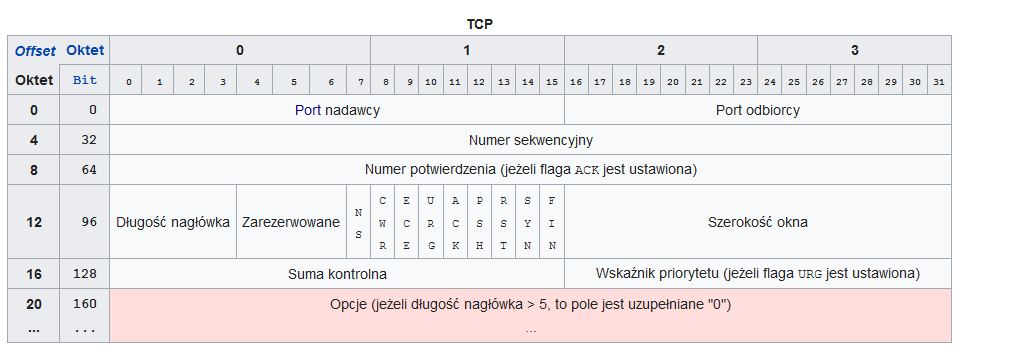
\includegraphics[width=\textwidth]{2.jpg}
\caption { Segment TCP, źródło: wilkiepedia.}
\end{figure}

\subsubsection{UDP}
Protokół transmisji danych,  dopuszczający pewne straty danych. Przez to ramka jest znacznie mniejsza, ukazuje to rys. \ref{zdj:4}). Protokól koncetruje się na szybkości dostarczenia pakietu.
\begin{figure}
\label{zdj:4}
\centering
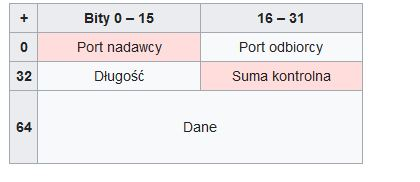
\includegraphics[width=\textwidth]{3.jpg}
\caption { nagłówek UDP, źródło: wilkiepedia.}
\end{figure}
\subsection{Diagramy sekwencji}
Przedstawiono następujące dogramy sekwencji:
\begin{itemize}
\item nawiązywanie połączenia (version, verack) grafika \ref{zdj:sek:version}
\item Uzyskiwania adresów ip z węzła(getaddr, addr) na grafice \ref{zdj:sek:getaddr}
\end{itemize}

\begin{figure}

\caption{Diagram sekwencji dla getaddr. Pominięto nawiązywanie połączenia(tcp, version,verack)}
\label{zdj:sek:getaddr}
\centering
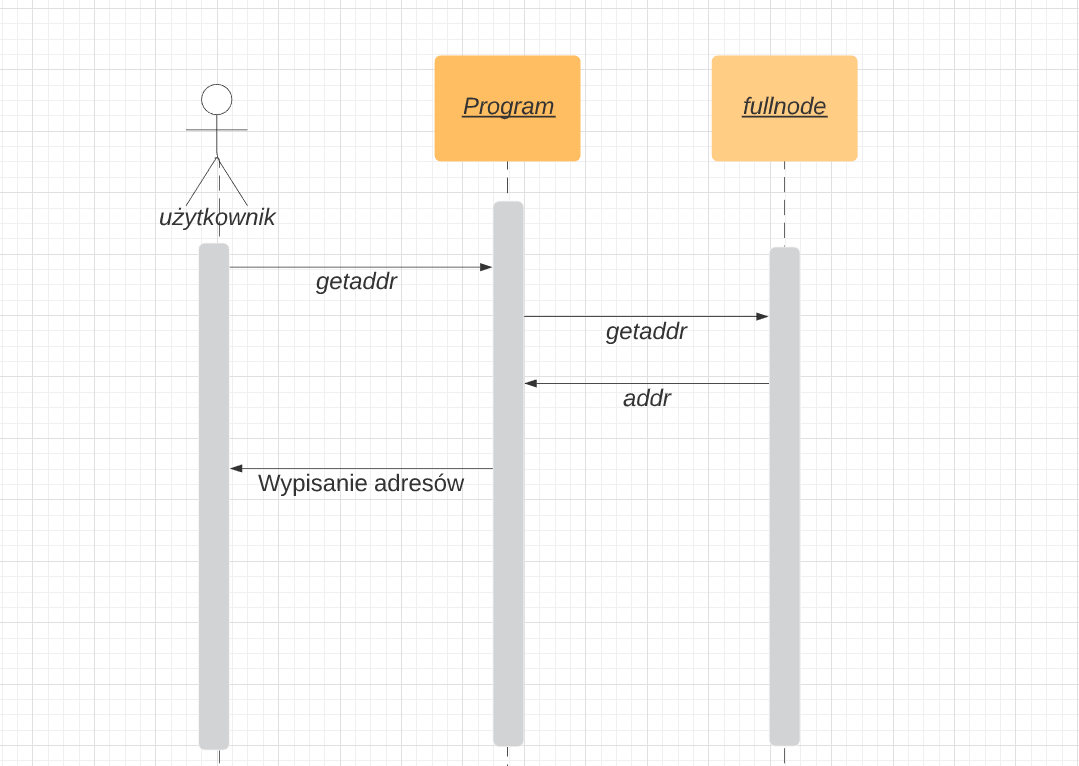
\includegraphics[width=\textwidth]{zdjecia/sekwencjiGetAddr}
\end{figure}

\begin{figure}

\caption{Diagram sekwencji dla nawiązywania połączenia(version,verack).}
\label{zdj:sek:version}
\centering
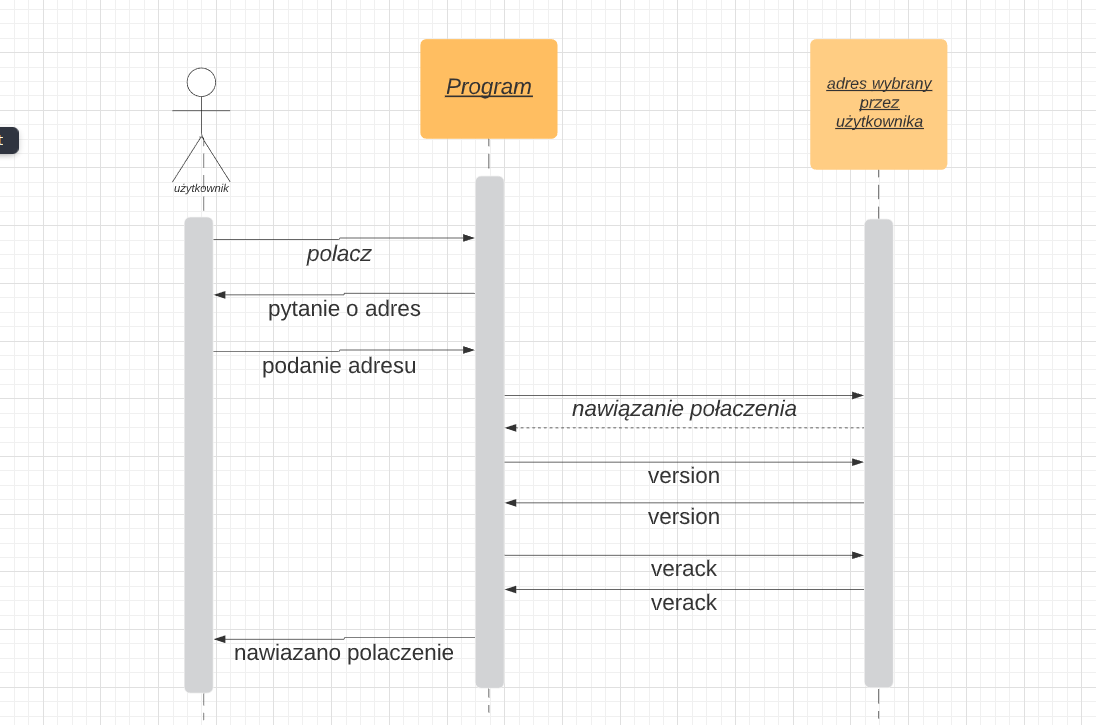
\includegraphics[width=\textwidth]{zdjecia/sekwencjiVersion}
\end{figure}
\section{FAQ}
\begin{itemize}
\item Dlaczego program nie działa?\\
Należy sprawdzić czy na komputerze zainstalowana jest odpowiednia wersja języka Python jak i systemu operacyjnego(patrz rozdział \autoref{chap:1}).
\item Czemu nie działa komunikacja z serwerem?\\
Sprawdź za pomocą polecenia ping czy istnieje połączenie, jeśli tak wpisz polecenie polacz. w innym przypadku skontatuj się z dostawcą internetu.
\item Czemu nie dzaiała polecenie?\\
Zweryfikuj czy jest to polecenie z "gwiazdką", jesli nie najpierw wpisz polecenie polacz.
\item Nie otrzymuje odpowiedzi na wiadomość version gdy używam UDP!\\
UDP często \textit{gubi} dane a wiadomość \textit{version} musi dojść w całości żeby otrzymać na nią odpowiedź. Jest to standardowe zachowanie i nie należy się nim przejmować.
\end{itemize}
\end{document}